\documentclass[12pt,a4paper]{article}
\usepackage{ctex}
\usepackage{amsmath,amssymb}
\usepackage{geometry}
\usepackage{graphicx}
\usepackage{caption}
\usepackage{subcaption}
\usepackage{indentfirst}
\usepackage{hyperref}
\geometry{a4paper, scale=0.8}

\title{四阶 B 样条曲线的绘制与交互控制实验报告}
\author{15 刘行}
\date{\today}

\begin{document}
    \maketitle

    \section{实验背景}
        在计算机图形学, CAD/CAM 系统, 动画制作, 工业设计以及 Office 办公软件中, 平滑曲线的生成是图形编辑的重要基础. 常见的曲线表示方法包括贝塞尔曲线, 样条插值曲线以及 B 样条 (B-Spline) 曲线等.
        B 样条曲线因其局部可控性, 良好的平滑性和较高的数值稳定性, 被广泛应用于曲线建模, 字体设计, 路径平滑, 数据可视化和用户界面控件绘制等领域.

        在本实验中, 我们实现了一个 \textbf{交互式 B 样条插值曲线编辑器}, 用户可以通过鼠标点击定义控制点, 生成对应的 B 样条控制点, 并实时观察 B 样条曲线的变化. 该程序完全使用 MATLAB 自编函数实现 B 样条的基函数与曲线生成过程, 未依赖内置样条函数.

    \section{实验原理}
        \subsection{B 样条曲线的定义}
            设有一组控制点
            \begin{equation*}
                P_0, P_1, \dots, P_{n-1} \in \mathbb{R}^2,
            \end{equation*}
            以及结点向量 (knot vector)
            \begin{equation*}
                t = \{t_0, t_1, \dots, t_{n+k}\}, \quad t_i \le t_{i+1},
            \end{equation*}
            则 $k$ 阶 (即次数为 $k-1$) B 样条曲线定义为
            \begin{equation*}
                C(u) = \sum_{i=0}^{n-1} N_{i,k}(u) \, P_i, \quad u \in [t_k,\, t_{n}].
            \end{equation*}
            其中 $N_{i,k}(u)$ 为 $k$ 阶 B 样条基函数, 满足分段多项式形式且局部支撑 (每个基函数只在 $[t_i, t_{i+k}]$ 上非零).

        \subsection{Cox-de Boor 递推公式}
            基函数 $N_{i,k}(u)$ 可由 Cox-de Boor 递推关系定义:
            \begin{equation*}
                N_{i,1}(u) =
            \begin{cases}
                1, & t_i \le u < t_{i+1}, \\
                0, & \text{otherwise,}
            \end{cases}
            \end{equation*}
            \begin{equation*}
                N_{i,k}(u) = \frac{u - t_i}{t_{i+k-1} - t_i} N_{i,k-1}(u) + \frac{t_{i+k} - u}{t_{i+k} - t_{i+1}} N_{i+1,k-1}(u).
            \end{equation*}

            这种递归定义保证了 B 样条曲线的以下性质:
            \begin{itemize}
                \item 基函数非负: $N_{i,k}(u) \ge 0$;
                \item 分片定义且局部支撑;
                \item 满足归一性: $\sum_i N_{i,k}(u) = 1$;
                \item 在结点向量边界处具有连续性 $C^{k-2}$.
            \end{itemize}

        \subsection{四阶 (即三次) B 样条}
            在本实验中取 $k=4$, 即曲线为三次 (cubic) B 样条.
            对应的结点向量构造为:
            \begin{equation*}
                t = [\underbrace{0, 0, 0, 0}_{k}, 1, 2, \dots, n-k, \underbrace{n-k+1, \dots, n-k+1}_{k}],
            \end{equation*}
            并归一化到 $[0,1]$ 区间:
            \begin{equation*}
                t \leftarrow \frac{t}{n-k+1}.
            \end{equation*}

            对于任意参数 $u \in [0,1]$, 可通过递归计算得到各基函数值, 再由线性组合公式求得曲线点:
            \begin{equation*}
                C(u) = \sum_{i=1}^{n} N_{i,4}(u) P_i.
            \end{equation*}

        \subsection{局部性与平滑性}
            每个基函数 $N_{i,4}(u)$ 仅在 $[t_i, t_{i+4}]$ 内非零, 因此移动某个控制点 $P_i$ 只会影响相邻 4 个区段上的曲线形状. 此外, 三次 B 样条具有 $C^2$ 连续性, 即曲线在连接处一阶, 二阶导数连续.

        \subsection{B 样条插值的原理}
            在前述定义中, B 样条曲线通常仅由控制点决定, 其轨迹一般不经过这些控制点.
            若希望曲线严格通过给定的数据点
            \begin{equation*}
                P_0, P_1, \dots, P_{n-1},
            \end{equation*}
            则需进行 \textbf{B 样条插值} (B-spline interpolation).

            设参数节点为
            \begin{equation*}
                u_0, u_1, \dots, u_{n-1},
            \end{equation*}
            插值条件为
            \begin{equation*}
                C(u_j) = P_j, \quad j = 0, 1, \dots, n-1.
            \end{equation*}
            由 B 样条定义式;
            \begin{equation*}
                C(u_j) = \sum_{i=0}^{n-1} N_{i,k}(u_j) \, Q_i,
            \end{equation*}
            其中 \( Q_i \) 为待求控制点. 由此可得线性方程组;
            \begin{equation*}
                A Q = P, \quad \text{其中 } A_{ji} = N_{i,k}(u_j).
            \end{equation*}
            解得控制点向量;
            \begin{equation*}
                Q = A^{-1} P.
            \end{equation*}
            将 $Q_i$ 代入标准 B 样条公式, 即可得到通过所有数据点的插值曲线.

            与传统的三次样条插值 (Cubic spline interpolation) 相比, B 样条插值具有如下优点:
            \begin{itemize}
                \item 系数矩阵 $A$ 具有带状结构, 数值稳定;
                \item 对局部数据变化响应平滑;
                \item 可自然推广至高维情形 (如曲面插值).
            \end{itemize}

        \subsection{参数化与结点向量的选择}
            插值结果的形状依赖于参数化方式与结点向量的分布.

            常见的参数化策略包括;
            \begin{itemize}
                \item \textbf{均匀参数化 (Uniform)}:
                    \begin{equation*}
                        u_j = \frac{j}{n-1},
                    \end{equation*}
                    简单但对点间距不敏感, 易产生波动;
                \item \textbf{弦长参数化 (Chord length)}:
                    \begin{equation*}
                        u_j =  \frac{\sum_{i=1}^{j} \|P_i - P_{i-1}\|}{\sum_{i=1}^{n-1} \|P_i - P_{i-1}\|},
                    \end{equation*}
                    能较好反映点间距离, 平滑且稳定;
                \item \textbf{中心偏差参数化 (Centripetal)}:
                    \begin{equation*}
                        u_j = \frac{\sum_{i=1}^{j} \|P_i - P_{i-1}\|^{1/2}}{\sum_{i=1}^{n-1} \|P_i - P_{i-1}\|^{1/2}},
                    \end{equation*}
                    可有效抑制密集点处的过拟合.
            \end{itemize}

            本实验采用弦长参数化方式, 以在平滑性与精确性之间取得较佳平衡.

            结点向量采用 \textbf{开放均匀结点} (open uniform knot vector):
            \begin{equation*}
                t = [\underbrace{0, \dots, 0}_{k}, \; t_k, t_{k+1}, \dots, t_{n-1}, \; \underbrace{1, \dots, 1}_{k}],
            \end{equation*}
            该结构保证曲线首尾通过首尾数据点, 并具有连续性 $C^{k-2}$.

    \section{代码实现}
        程序由 MATLAB 实现, 核心部分包括以下几个函数:

        \begin{itemize}
            \item \textbf{drawpolyline}: 交互式绘制控制点序列, 用户点击鼠标添加锚点并按回车结束输入;
            \item \textbf{addlistener}: 为控制点的移动事件绑定监听器, 实现拖动控制点时曲线的实时更新;
            \item \textbf{bspline\_basis(i, k, t, u)}: 递归计算 $N_{i,k}(u)$;
            \item \textbf{bspline\_point(P, k, t, u)}: 计算给定参数 $u$ 的曲线点;
            \item \textbf{plotBSpline(P)}: 遍历参数区间, 计算并绘制整条 B 样条曲线.
        \end{itemize}

        程序结构如下:
        \begin{verbatim}
main
 |- plotBSpline
 |    |- bspline_point
 |    |    \- bspline_basis (递归)
 \- updateBSpline (事件回调)
        \end{verbatim}

    \section{使用方法}
        \begin{enumerate}
            \item 运行主函数 \texttt{main};
            \item 在图形窗口中依次点击以添加锚点;
            \item 按下回车键结束点的输入;
            \item 系统自动绘制 B 样条曲线;
            \item 拖动任意控制点, 曲线将实时更新.
        \end{enumerate}

    \section{实验结果与效果展示}
        程序运行后可获得如下效果: 黑色折线为控制多边形, 红色虚折线为对应 B 样条控制多边形, 蓝色曲线为对应的三次 B 样条. 用户拖动控制点时, 曲线平滑地变化, 验证了 B 样条插值的局部可控性和平滑性.

        \begin{figure}[ht]
            \centering
            \begin{minipage}[t]{0.48\textwidth}
                \centering
                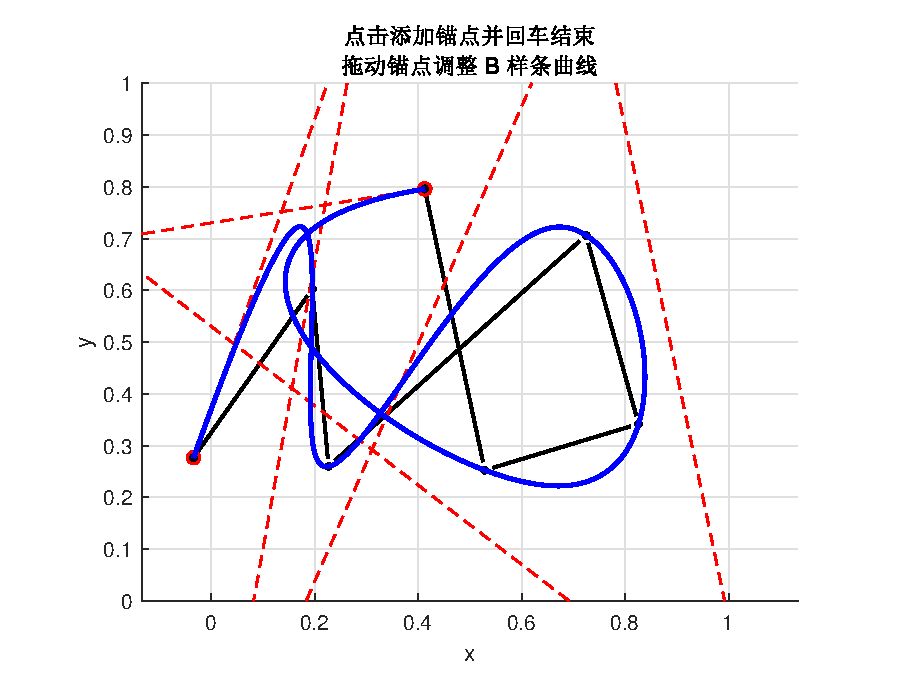
\includegraphics[width=\textwidth]{fig/result01.eps}
                \caption*{(a) 初始曲线}
            \end{minipage}
            \hfill
            \begin{minipage}[t]{0.48\textwidth}
                \centering
                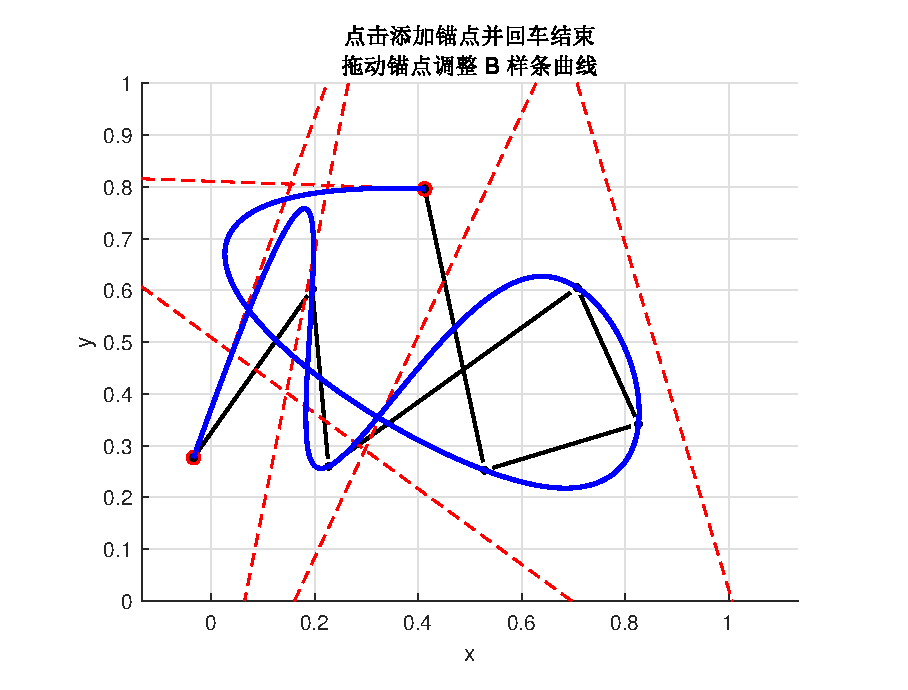
\includegraphics[width=\textwidth]{fig/result02.eps}
                \caption*{(b) 调整后的曲线}
            \end{minipage}
            \caption{四阶 B 样条插值曲线交互绘制结果}
            \label{fig:result}
        \end{figure}

    \section{结论}
        本实验手动实现了四阶 B 样条插值曲线的绘制与交互控制过程, 验证了 B 样条插值曲线的以下性质:
        \begin{itemize}
            \item 曲线在控制点附近平滑可控;
            \item 满足 $C^2$ 连续性;
            \item 对控制点移动具有局部响应;
            \item 计算稳定, 实现简洁.
        \end{itemize}

        本程序可作为计算机图形学中曲线造型, 路径拟合及 CAD 编辑系统的基础模块, 具有较好的实用价值和扩展潜力.
\end{document}
